%
% $RCSfile: single_model.tex,v $
%
% Copyright (C) 2002-2008. Christian Heller.
%
% Permission is granted to copy, distribute and/or modify this document
% under the terms of the GNU Free Documentation License, Version 1.1 or
% any later version published by the Free Software Foundation; with no
% Invariant Sections, with no Front-Cover Texts and with no Back-Cover
% Texts. A copy of the license is included in the section entitled
% "GNU Free Documentation License".
%
% http://www.cybop.net
% - Cybernetics Oriented Programming -
%
% http://www.resmedicinae.org
% - Information in Medicine -
%
% Version: $Revision: 1.1 $ $Date: 2008-08-19 20:41:08 $ $Author: christian $
% Authors: Christian Heller <christian.heller@tuxtax.de>
%

\subsubsection{Single Model}
\label{single_model_heading}
\index{Single Model Approach}
\index{Entity Relationship Model}
\index{ERM}
\index{Object Oriented Model}
\index{OOM}
\index{Unified Modelling Language}
\index{UML}

Today, the most common design approach for standard application software is to
create a \emph{Single Model} of types whose semantics is often described in
form of an \emph{Entity Relationship-} (ER) or \emph{Object Oriented} (OO)
model,
%(section \ref{data_model_heading}),
the latter sometimes illustrated
using diagrams of the \emph{Unified Modeling Language} (UML).

\begin{figure}[ht]
    \begin{center}
        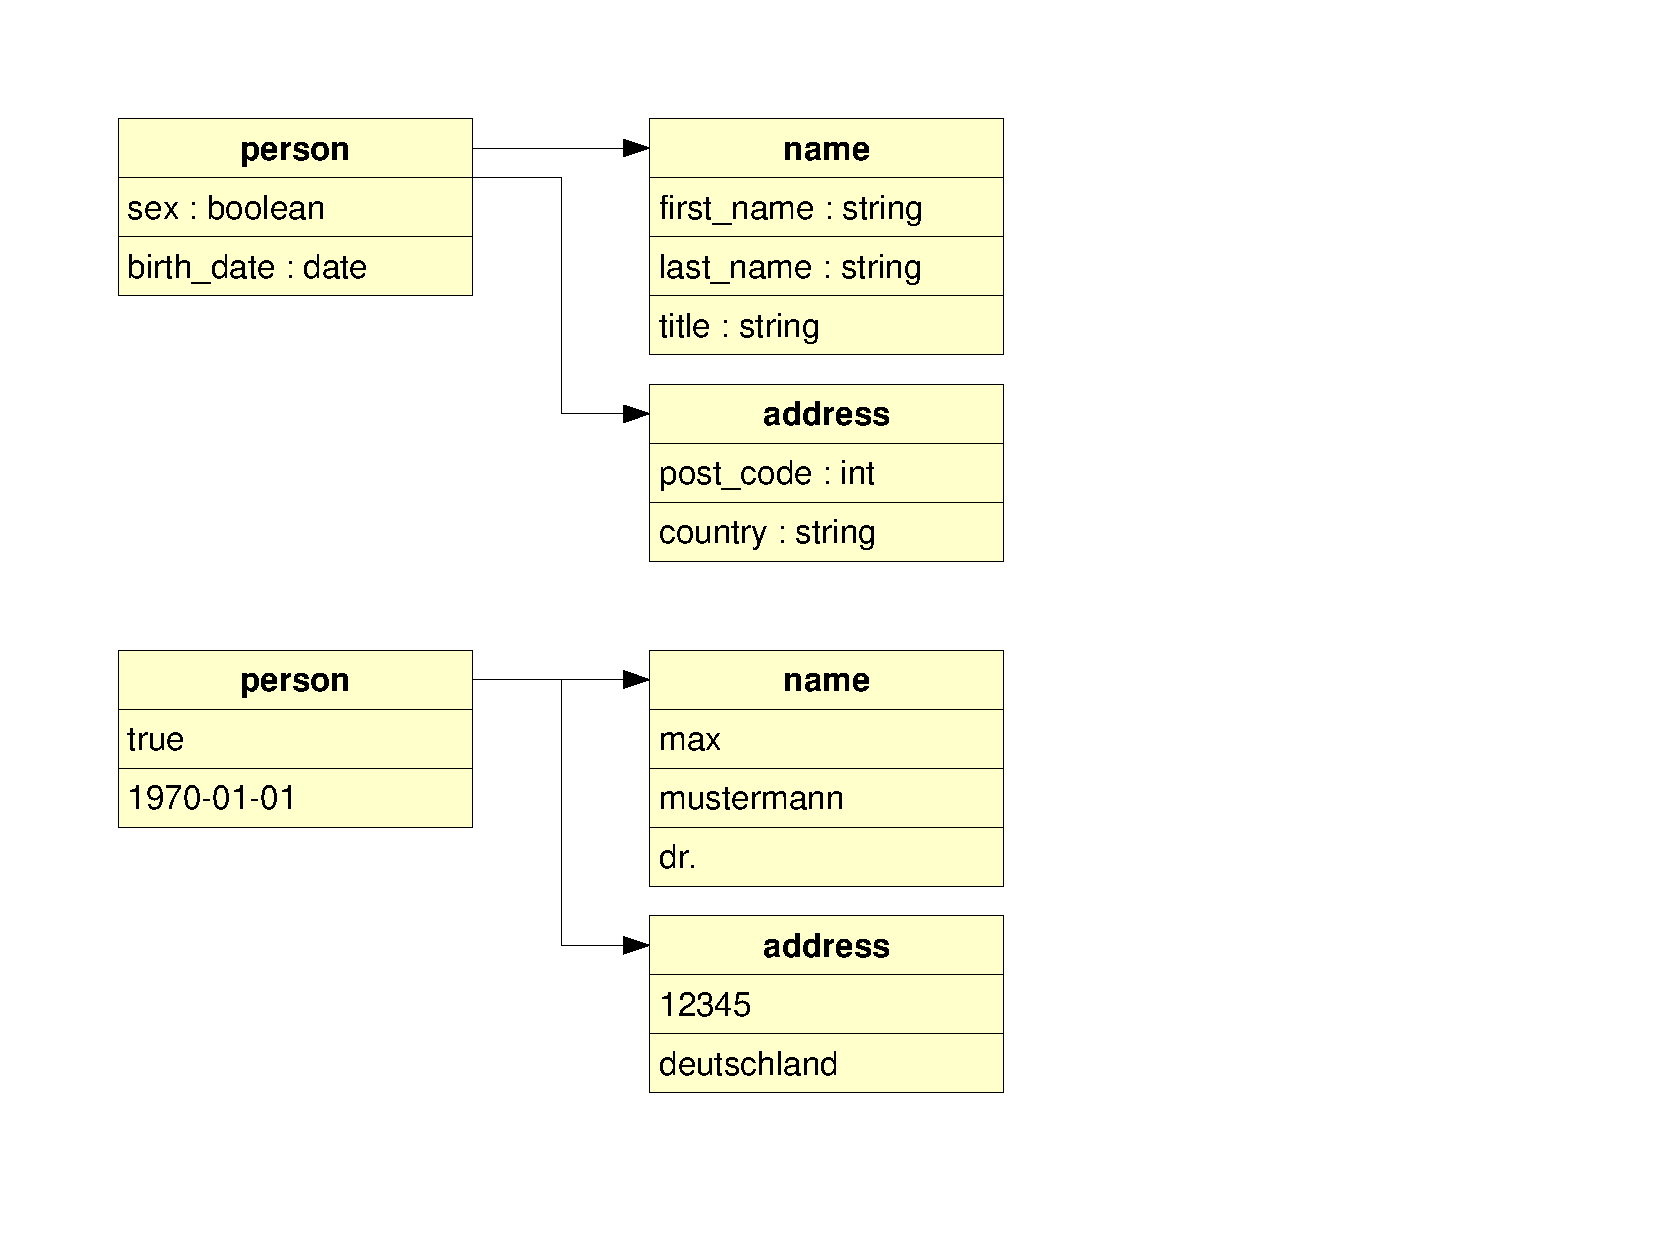
\includegraphics[scale=0.3,angle=-90]{graphic/single.pdf}
        \caption{Single Model Approach (adapted from \cite{archetypes})}
        \label{single_figure}
    \end{center}
\end{figure}

As example, figure \ref{single_figure} shows a UML \emph{Class Diagram} (CsD).
In its upper half, one can see a class \emph{Person} associated with the
classes \emph{Name} and \emph{Address}, as modelled at design time. They may be
part of a much larger model. The lower half of the figure shows the objects
(instances) at runtime, filled with concrete values. There are a number of
problems with this approach:

%
% $RCSfile: inflexible_architecture.tex,v $
%
% Copyright (C) 2002-2008. Christian Heller.
%
% Permission is granted to copy, distribute and/or modify this document
% under the terms of the GNU Free Documentation License, Version 1.1 or
% any later version published by the Free Software Foundation; with no
% Invariant Sections, with no Front-Cover Texts and with no Back-Cover
% Texts. A copy of the license is included in the section entitled
% "GNU Free Documentation License".
%
% http://www.cybop.net
% - Cybernetics Oriented Programming -
%
% http://www.resmedicinae.org
% - Information in Medicine -
%
% Version: $Revision: 1.1 $ $Date: 2008-08-19 20:41:07 $ $Author: christian $
% Authors: Christian Heller <christian.heller@tuxtax.de>
%

\paragraph{Inflexible Architecture}
\label{inflexible_architecture_heading}
\index{Inflexible Architecture}

First and foremost, the static coupling of classes leads to an inflexible
design. The names and number of attributes and methods as integral part of a
class cannot be changed dynamically later-on; only their values can. The class
structure represents a solution to a current problem. If it is static, then
future requirements cannot be considered. Adaptation issues and workarounds,
affecting stability and security, are thus to be expected.

%
% $RCSfile: concept_mix.tex,v $
%
% Copyright (C) 2002-2008. Christian Heller.
%
% Permission is granted to copy, distribute and/or modify this document
% under the terms of the GNU Free Documentation License, Version 1.1 or
% any later version published by the Free Software Foundation; with no
% Invariant Sections, with no Front-Cover Texts and with no Back-Cover
% Texts. A copy of the license is included in the section entitled
% "GNU Free Documentation License".
%
% http://www.cybop.net
% - Cybernetics Oriented Programming -
%
% http://www.resmedicinae.org
% - Information in Medicine -
%
% Version: $Revision: 1.1 $ $Date: 2008-08-19 20:41:06 $ $Author: christian $
% Authors: Christian Heller <christian.heller@tuxtax.de>
%

\paragraph{Concept Mix}
\label{concept_mix_heading}
\index{Concept Mix}

Further, specialised domain concepts identified during requirements analysis
(such as a \emph{Patient} being a kind of \emph{Person}) are often mixed up
with more general concepts as found during design (for example the application
of a proper \emph{Role} architecture instead of simple inheritance for the
person-patient relation). The lack of a proper separation between pure domain
knowledge (like a patient receiving a medication) and system control software
(like logging facilities or persistence mechanisms) was already explained in
detail in the previous chapter \ref{statics_and_dynamics_heading}. It frequently
leads to strong coupling between system layers and complicates software design.

%
% $RCSfile: synchronisation_problems.tex,v $
%
% Copyright (C) 2002-2008. Christian Heller.
%
% Permission is granted to copy, distribute and/or modify this document
% under the terms of the GNU Free Documentation License, Version 1.1 or
% any later version published by the Free Software Foundation; with no
% Invariant Sections, with no Front-Cover Texts and with no Back-Cover
% Texts. A copy of the license is included in the section entitled
% "GNU Free Documentation License".
%
% http://www.cybop.net
% - Cybernetics Oriented Programming -
%
% http://www.resmedicinae.org
% - Information in Medicine -
%
% Version: $Revision: 1.1 $ $Date: 2008-08-19 20:41:09 $ $Author: christian $
% Authors: Christian Heller <christian.heller@tuxtax.de>
%

\paragraph{Synchronisation Problems}
\label{synchronisation_problems_heading}
\index{Synchronisation Problems}

The mix of application knowledge with system control software also causes
synchronisation (communication) problems within software development projects.
Domain experts and software developers depend on each other: Developers need to
first understand domain knowledge before being able to correctly implement it
into software. Experts bring their knowledge into a more software-friendly
form, during analysis.

%
% $RCSfile: complicated_processing.tex,v $
%
% Copyright (C) 2002-2008. Christian Heller.
%
% Permission is granted to copy, distribute and/or modify this document
% under the terms of the GNU Free Documentation License, Version 1.1 or
% any later version published by the Free Software Foundation; with no
% Invariant Sections, with no Front-Cover Texts and with no Back-Cover
% Texts. A copy of the license is included in the section entitled
% "GNU Free Documentation License".
%
% http://www.cybop.net
% - Cybernetics Oriented Programming -
%
% http://www.resmedicinae.org
% - Information in Medicine -
%
% Version: $Revision: 1.1 $ $Date: 2008-08-19 20:41:06 $ $Author: christian $
% Authors: Christian Heller <christian.heller@tuxtax.de>
%

\paragraph{Complicated Processing}
\label{complicated_processing_heading}
\index{Complicated Processing}
\index{Data Mining}
\index{Decision Support}

Due to the great variety of software architectures, it is pretty hard to
capture and process data from different systems in a uniform way, for reasons
of \emph{Data Mining}, for example. Unpredictable architecture changes caused
by new domain requirements hamper the creation of reliable rules for
\emph{Decision Support}.

%
% $RCSfile: steady_upgrading.tex,v $
%
% Copyright (C) 2002-2008. Christian Heller.
%
% Permission is granted to copy, distribute and/or modify this document
% under the terms of the GNU Free Documentation License, Version 1.1 or
% any later version published by the Free Software Foundation; with no
% Invariant Sections, with no Front-Cover Texts and with no Back-Cover
% Texts. A copy of the license is included in the section entitled
% "GNU Free Documentation License".
%
% http://www.cybop.net
% - Cybernetics Oriented Programming -
%
% http://www.resmedicinae.org
% - Information in Medicine -
%
% Version: $Revision: 1.1 $ $Date: 2008-08-19 20:41:09 $ $Author: christian $
% Authors: Christian Heller <christian.heller@tuxtax.de>
%

\paragraph{Steady Upgrading}
\label{steady_upgrading_heading}
\index{Steady Upgrading}

Applications that were designed in a \emph{Single Model} manner require steady
upgrading. Whenever new domain knowledge gets worked into the system or
existing knowledge gets adapted to new requirements, the software design may
change -- even in important parts that would better remain stable. Accordingly,
systems of that kind cannot be labelled \emph{future-proof}.

%
% $RCSfile: no_standardisation.tex,v $
%
% Copyright (C) 2002-2008. Christian Heller.
%
% Permission is granted to copy, distribute and/or modify this document
% under the terms of the GNU Free Documentation License, Version 1.1 or
% any later version published by the Free Software Foundation; with no
% Invariant Sections, with no Front-Cover Texts and with no Back-Cover
% Texts. A copy of the license is included in the section entitled
% "GNU Free Documentation License".
%
% http://www.cybop.net
% - Cybernetics Oriented Programming -
%
% http://www.resmedicinae.org
% - Information in Medicine -
%
% Version: $Revision: 1.1 $ $Date: 2008-08-19 20:41:07 $ $Author: christian $
% Authors: Christian Heller <christian.heller@tuxtax.de>
%

\paragraph{No Standardisation}
\label{no_standardisation_heading}
\index{Difficult Standardisation of Software Models}

Finally, a true standardisation of single model systems is hardly reachable.
Requirements are just too different between the systems, and they change much
too often. A standard architecture of that kind won't remain stable for very
long.

